\documentclass{article}

%
% 引入模板的style文件
%
\usepackage{homework}

\setCJKmainfont{SimSun}[AutoFakeBold] %宋体加粗
\setCJKsansfont{SimHei}[AutoFakeBold] %黑体加粗


\usepackage{minted} %配合minted宏包进行好看的高亮
\usepackage{currfile} %配合minted宏包进行好看的高亮
\usepackage{caption} %配合minted宏包进行好看的高亮
\usepackage{tcolorbox} %配合minted宏包进行好看的高亮
\usepackage{xcolor} %配合minted宏包进行好看的高亮
\tcbuselibrary{skins} %配合minted宏包进行好看的高亮
\tcbuselibrary{minted} %配合minted宏包进行好看的高亮
\usemintedstyle{paraiso-dark} %配合minted宏包进行好看的高亮
\usepackage{framed} 
\usepackage{amsmath}

\usepackage{graphicx}
\usepackage{float}
\usepackage{subfig}


%
% 封面
%


\title{
	
\includegraphics[width=0.6\textwidth]{images/title/ucas_logo 1.pdf}\\
    \vspace{1in}
    \textmd{\textbf{\hmwkClass}}\\
	\textmd{\Large{\textbf{\hmwkClassID}}}\\
    \textmd{\textbf{\hmwkTitle}}\\
    \normalsize\vspace{0.1in}\large{\hmwkCompleteTime }\\
    \vspace{0.1in}\large{\textit{\hmwkClassInstructor\ }}\\
    \vspace{1in}
	
\includegraphics[width=0.25\textwidth]{images/title/Cyber.jpg}\\
	\vspace{1in}
}

\author{
	\hmwkAuthorName \\ 
	\hmwkAuthorStuID \\
	\hmwkAuthorInst \\
	\hmwkAuthorzhuanye \\
	\hmwkAuthorfangxiang
	}
\date{}

\renewcommand{\part}[1]{\textbf{\large Part \Alph{partCounter}}\stepcounter{partCounter}\\}


%
% 正文部分
%
\begin{document}


\maketitle


%\include{chapters/ch01}
%\include{chapters/ch02}
%\include{chapters/ch03}
%\include{chapters/ch04}
%\include{chapters/ch05}


\pagebreak

\begin{homeworkProblem}
	设计一个Las Vegas随机算法, 求解电路板布线问题. 将该算法与分支限界算法结合, 观察求解效率.

	\solution 该算法的设计核心是: \textbf{采用随机放置位置策略并结合分支限界算法}. 算法的C++代码如下所示: 
\begin{tcblisting}{listing engine=minted,boxrule=0.1mm,
colback=blue!5!white,colframe=blue!75!black,
listing only,left=5mm,enhanced,sharp corners=all,
overlay={\begin{tcbclipinterior}\fill[red!20!blue!20!white] (frame.south west)
rectangle ([xshift=5mm]frame.north west);\end{tcbclipinterior}},
minted language=c++,
minted style=tango,
minted options={fontsize=\small,breaklines,autogobble,linenos,numbersep=3mm}}
#include <bits/stdc++.h> //万能头文件, 刷题时可以用, 大型项目千万不能用
using namespace std;

//表示方格位置上的结构体
struct position{
    int row;
    int col;
};

//分支限界算法
bool FindPath(
    position start, position finish, int &PathLen,
    position *&path, int **grid, int m, int n
) { //找到最短布线路径, 若找得到则返回true, 否则返回false
    //起点终点重合则不用布线
    if((start.row == finish.row) && (start.col == finish.col)) {
        PathLen = 0;
        return true;
    }

    //设置方向移动坐标值: 东南西北
    position offset[4];
    offset[0].row = 0;
    offset[0].col = 1; //右移
    offset[1].row = 1;
    offset[1].col = 0; //下移
    offset[2].row = 0;
    offset[2].col = -1; //左移
    offset[3].row = -1;
    offset[3].col = 0; //上移

    int NumNeighBlo = 4; //相邻的方格数
    position here, nbr;
    here.row = start.row; //设置当前方格, 即搜索单位
    here.col = start.col;
    //由于0和1用于表示方格的开放和封闭, 故距离: 2-0 3-1
    grid[start.row][start.col] = 0; //-2表示强, -1表示可行, -3表示不能当作路线
    //队列式搜索, 标记可达相邻方格
    queue<position> q_FindPath;
\end{tcblisting}
\begin{tcblisting}{listing engine=minted,boxrule=0.1mm,
colback=blue!5!white,colframe=blue!75!black,
listing only,left=5mm,enhanced,sharp corners=all,
overlay={\begin{tcbclipinterior}\fill[red!20!blue!20!white] (frame.south west)
rectangle ([xshift=5mm]frame.north west);\end{tcbclipinterior}},
minted language=c++,
minted style=tango,
minted options={fontsize=\small,breaklines,autogobble,linenos,numbersep=3mm}}
    do {
        int num = 0; //方格未标记个数
        position selectPosition[5]; //保存选择位置
        for(int i = 0; i < NumNeighBlo; i++) {
            //到达四个方向
            nbr.row = here.row + offset[i].row;
            nbr.col = here.col + offset[i].col;
            if(grid[nbr.row][nbr.col] == -1) { //该方格未标记
                grid[nbr.row][nbr.col] = grid[here.row][here.col] + 1;
                if((nbr.row == finish.row) && (nbr.col == finish.col)) {
                    break;
                }
                selectPosition[num].row = nbr.row;
                selectPosition[num].col = nbr.col;
                num++;
            }
        }
        if(num > 0) { //如果标记, 则在这么多个未标记个数中随机选择一个位置(本算法核心)
            q_FindPath.push(selectPosition[rand()%(num)]); //随机选一个入队
        }
        if((nbr.row == finish.row) && (nbr.col == finish.col)) {
            break; //是否到达目标位置finish
        }
        //判断活结点队列是否为空
        if(q_FindPath.empty() == true) return false; // 无解
        //访问队首元素出队
        here = q_FindPath.front();
        q_FindPath.pop();
    } while (true);

    //构造最短布线路径
    PathLen = grid[finish.row][finish.col];
    path = new position[PathLen]; //路径
    //从目标位置finish开始向起始位置回溯
    here = finish;
    for(int j = PathLen - 1; j >= 0; j--) {
        path[j] = here;
        //找前驱位置
        for(int i = 0; i <= NumNeighBlo; i++) {
            nbr.row = here.row + offset[i].row;
            nbr.col = here.col + offset[i].col;
            if(grid[nbr.row][nbr.col] == j) {//距离+2正好是前驱位置
                break;
            }
        }
        here = nbr;
    }
    return true;
}
\end{tcblisting}
\begin{tcblisting}{listing engine=minted,boxrule=0.1mm,
colback=blue!5!white,colframe=blue!75!black,
listing only,left=5mm,enhanced,sharp corners=all,
overlay={\begin{tcbclipinterior}\fill[red!20!blue!20!white] (frame.south west)
rectangle ([xshift=5mm]frame.north west);\end{tcbclipinterior}},
minted language=c++,
minted style=tango,
minted options={fontsize=\small,breaklines,autogobble,linenos,numbersep=3mm}}
int main() {
    cout << "---------分支限界算法之布线问题---------" << endl;
    int path_len, path_len1, m, n;
    position *path, *path1, start, finish, start1, finish1;
    cout << "在一个m*n的棋盘上, 请分别输入m和n, 代表行数和列数, 然后输入回车" << endl;
    cin >> m >> n;
    //创建棋盘格
    int **grid = new int * [m + 2], **grid1 = new int * [m + 2];
    for(int i = 0; i < m + 2; i++) {
        grid[i] = new int[n + 2];
        grid1[i] = new int[n + 2];
    }
    //初始化棋盘
    for(int i = 1; i <= m; i++) {
        for(int j = 1; j <= n; j++) {
            grid[i][j] = -1;
        }
    }
    //设置方格阵列的围墙
    for(int i = 0; i <= n + 1; i++) {
        grid[0][i] = grid[m + 1][i] = -2; //上下的围墙
    }
    for(int i = 0; i <= m + 1; i++) {
        grid[i][0] = grid[i][n + 1] = -2; //左右的围墙
    }
    cout << "初始化棋盘格和加围墙" << endl;
    cout << "------------------" << endl;
    for(int i = 0; i < m + 2; i++) {
        for(int j = 0; j < n + 2; j++) {
            cout << grid[i][j] << " ";
        }
        cout << endl;
    }
    cout << "------------------" << endl;
    cout << "请输入已经占据的位置(行坐标, 列坐标), 代表此位置不能布线" << endl;
    cout << "例如输入2 2(然后输入回车), 表示坐标(2,2)不能布线;" <<
    "当输入坐标为0 0(然后输入回车)表示结束输入" << endl;
    //添加已经布线的棋盘格
    while(true) {
        int ci, cj;
        cin >> ci >> cj;
        if(ci > m || cj > n) {
            cout << "输入非法!";
            cout << "行坐标<" << m << ", 列坐标<" << n << "当输入的坐标为0,0时结束输入" << endl;
            continue;
        } else if (ci == 0 || cj == 0) {
            break;
        } else {
            grid[ci][cj] = -3;
        }
    }
\end{tcblisting}
\begin{tcblisting}{listing engine=minted,boxrule=0.1mm,
colback=blue!5!white,colframe=blue!75!black,
listing only,left=5mm,enhanced,sharp corners=all,
overlay={\begin{tcbclipinterior}\fill[red!20!blue!20!white] (frame.south west)
rectangle ([xshift=5mm]frame.north west);\end{tcbclipinterior}},
minted language=c++,
minted style=tango,
minted options={fontsize=\small,breaklines,autogobble,linenos,numbersep=3mm}}
    //布线前的棋盘格
    cout << "布线前的棋盘格" << endl;
    cout << "------------------" << endl;
    for(int i = 0; i < m + 2; i++) {
        for(int j = 0; j < n + 2; j++) {
            cout << grid[i][j] << " ";
        }
        cout << endl;
    }
    cout << "------------------" << endl;
    cout << "请输入起点位置坐标" << endl;
    cin >> start.row >> start.col;
    cout << "请输入终点位置坐标" << endl;
    cin >> finish.row >> finish.col;
    clock_t starttime, endtime;
    starttime = clock(); //程序开始时间
    srand((unsigned) time (NULL)); //初始化时间种子, 是随机选择的关键
    int time = 0; //为假设运行次数
    start1 = start, finish1 = finish, path_len1 = path_len, path1 = NULL; //初始值拷贝
    for(int i = 0; i < m + 2; i++) {
        for(int j = 0; j < n + 2; j++) {
            grid1[i][j] = grid[i][j];
        }
    }
    bool result = FindPath(start1, finish1, path_len1, path1, grid1, m, n);
    while(result == 0 && time < 1000) { //尝试次数最多为1000次
        //初始值拷贝
        start1 = start, finish1 = finish, path_len1 = path_len, path1 = NULL;
        for(int i = 0; i < m + 2; i++) {
            for(int j = 0; j < n + 2; j++) {
                grid1[i][j] = grid[i][j];
            }
        }
        time++;
        cout << endl;
        cout << "没有找到路线, 第" << time << "次尝试" << endl;
        result = FindPath(start1, finish1, path_len1, path1, grid1, m, n);
    }
    endtime = clock(); //程序结束时间

    if(result == 1) {
        cout << "------------------" << endl;
        cout << "$ 代表围墙" << endl;
        cout << "# 代表已经占据的点" << endl;
        cout << "* 代表布线路线" << endl;
        cout << "= 代表还没有布线的点" << endl;
        cout << "------------------" << endl;
        for(int i = 0; i <= m + 1; i++) {
            for(int j = 0; j <= n + 1; j++) {
                if(grid1[i][j] == -2) cout << "$ ";
                else if(grid1[i][j] == -3) cout << "# ";
\end{tcblisting}

\begin{tcblisting}{listing engine=minted,boxrule=0.1mm,
colback=blue!5!white,colframe=blue!75!black,
listing only,left=5mm,enhanced,sharp corners=all,
overlay={\begin{tcbclipinterior}\fill[red!20!blue!20!white] (frame.south west)
rectangle ([xshift=5mm]frame.north west);\end{tcbclipinterior}},
minted language=c++,
minted style=tango,
minted options={fontsize=\small,breaklines,autogobble,linenos,numbersep=3mm}}
                else {
                    int r;
                    for(r = 0; r < path_len1; r++) {
                        if(i == path1[r].row && j == path1[r].col) {
                            cout << "* ";
                            break;
                        }
                        if(i == start1.row && j == start1.col) {
                            cout << "* ";
                            break;
                        }
                    }
                    if(r == path_len1) cout << "= ";
                }
            }
            cout << endl;
        }
        cout << "------------------" << endl;
        cout << "路径坐标和长度" << endl;
        cout << endl;
        cout << "(" << start1.row << "," << start1.col << ")" << " ";
        for(int i = 0; i < path_len1; i++) {
            cout << "(" << path1[i].row << "," << path1[i].col << ")" << " ";
        }
        cout << endl;
        cout << endl;
        cout << "路径长度: " << path_len1 + 1 << endl;
        cout << endl;
        time++;
        cout << "布线完毕, 共查找" << time << "次" << endl;
        cout << "算法运行时间为: " << (endtime - starttime) << "ms" << endl;
    } else {
        cout << endl;
        cout << "经过多次尝试, 依然没有找到路线" << endl;
    }
    return 0;
}
\end{tcblisting}
	上述代码的关键之处在于:
	\begin{itemize}
		\item P3页的第13行代码, 这里是当前点相邻四个点是否可以放置, 如果可以放置用selectPostion保存下来, 并用num记录有多少个位置可以放置;
		\item P3页的第19行代码, 这里利用上面保存的可以放置的点, 然后\textbf{随机选取其中一个加入队列}, 这就是Las Vegas算法的精髓;
		\item P5页的第17行代码, 作用是初始化时间种子, 是伪随机生成器的关键, 即是随机选择的关键.
	\end{itemize}
	\textbf{结果分析:}
	\begin{itemize}
		\item 测试样例1: $3\times 3$棋盘, 代码的交互输出过程如下:
\begin{tcblisting}{listing engine=minted,boxrule=0.1mm,
colback=blue!5!white,colframe=blue!75!black,
listing only,left=5mm,enhanced,sharp corners=all,
overlay={\begin{tcbclipinterior}\fill[red!20!blue!20!white] (frame.south west)
rectangle ([xshift=5mm]frame.north west);\end{tcbclipinterior}},
minted language=c++,
minted style=tango,
minted options={fontsize=\small,breaklines,autogobble,linenos,numbersep=3mm}}
开始运行...
---------分支限界算法之布线问题---------
在一个m*n的棋盘上, 请分别输入m和n, 代表行数和列数, 然后输入回车
3 3
初始化棋盘格和加围墙
------------------
-2 -2 -2 -2 -2 
-2 -1 -1 -1 -2 
-2 -1 -1 -1 -2 
-2 -1 -1 -1 -2 
-2 -2 -2 -2 -2 
------------------
请输入已经占据的位置(行坐标, 列坐标), 代表此位置不能布线
例如输入2 2(然后输入回车), 表示坐标(2,2)不能布线;当输入坐标为0 0(然后输入回车)表示结束输入
2 1
2 3
3 3
0 0
布线前的棋盘格
------------------
-2 -2 -2 -2 -2 
-2 -1 -1 -1 -2 
-2 -3 -1 -3 -2 
-2 -1 -1 -3 -2 
-2 -2 -2 -2 -2 
------------------
请输入起点位置坐标
1 1
请输入终点位置坐标
3 1

没有找到路线, 第1次尝试

没有找到路线, 第2次尝试
------------------
$ 代表围墙
# 代表已经占据的点
* 代表布线路线
= 代表还没有布线的点
------------------
$ $ $ $ $ 
$ * * = $ 
$ # * # $ 
$ * * # $ 
$ $ $ $ $ 
------------------
路径坐标和长度
(1,1) (1,2) (2,2) (3,2) (3,1) 
路径长度: 5
布线完毕, 共查找3次
算法运行时间为: 39ms
运行结束.
\end{tcblisting}
	\item 测试样例2: $5\times 5$棋盘, 代码的交互输出过程如下:
\begin{tcblisting}{listing engine=minted,boxrule=0.1mm,
colback=blue!5!white,colframe=blue!75!black,
listing only,left=5mm,enhanced,sharp corners=all,
overlay={\begin{tcbclipinterior}\fill[red!20!blue!20!white] (frame.south west)
rectangle ([xshift=5mm]frame.north west);\end{tcbclipinterior}},
minted language=c++,
minted style=tango,
minted options={fontsize=\small,breaklines,autogobble,linenos,numbersep=3mm}}
---------分支限界算法之布线问题---------
在一个m*n的棋盘上, 请分别输入m和n, 代表行数和列数, 然后输入回车
5 5
请输入已经占据的位置(行坐标, 列坐标), 代表此位置不能布线
例如输入2 2(然后输入回车), 表示坐标(2,2)不能布线;当输入坐标为0 0(然后输入回车)表示结束输入
3 1
3 2
3 4
3 5
4 5
0 0
布线前的棋盘格
------------------
-2 -2 -2 -2 -2 -2 -2 
-2 -1 -1 -1 -1 -1 -2 
-2 -1 -1 -1 -1 -1 -2 
-2 -3 -3 -1 -3 -3 -2 
-2 -1 -1 -1 -1 -3 -2 
-2 -1 -1 -1 -1 -1 -2 
-2 -2 -2 -2 -2 -2 -2 
------------------
请输入起点位置坐标
1 1
请输入终点位置坐标
5 2
没有找到路线, 第1次尝试
没有找到路线, 第2次尝试
没有找到路线, 第3次尝试
------------------
$ 代表围墙
# 代表已经占据的点
* 代表布线路线
= 代表还没有布线的点
------------------
$ $ $ $ $ $ $ 
$ * = = = = $ 
$ * * * = = $ 
$ # # * # # $ 
$ = = * = # $ 
$ = * * = = $ 
$ $ $ $ $ $ $ 
------------------
路径坐标和长度
(1,1) (2,1) (2,2) (2,3) (3,3) (4,3) (5,3) (5,2) 
路径长度: 8
布线完毕, 共查找4次
算法运行时间为: 61ms
\end{tcblisting}
	\item 测试样例2: $10\times 10$棋盘, 代码的交互输出过程如下:
\begin{tcblisting}{listing engine=minted,boxrule=0.1mm,
colback=blue!5!white,colframe=blue!75!black,
listing only,left=5mm,enhanced,sharp corners=all,
overlay={\begin{tcbclipinterior}\fill[red!20!blue!20!white] (frame.south west)
rectangle ([xshift=5mm]frame.north west);\end{tcbclipinterior}},
minted language=c++,
minted style=tango,
minted options={fontsize=\small,breaklines,autogobble,linenos,numbersep=3mm}}
---------分支限界算法之布线问题---------
在一个m*n的棋盘上, 请分别输入m和n, 代表行数和列数, 然后输入回车
10 10
布线前的棋盘格
------------------
-2 -2 -2 -2 -2 -2 -2 -2 -2 -2 -2 -2 
-2 -1 -1 -1 -1 -1 -1 -1 -1 -1 -1 -2 
-2 -1 -1 -1 -1 -1 -1 -1 -1 -1 -1 -2 
-2 -1 -1 -1 -1 -1 -1 -1 -1 -1 -1 -2 
-2 -1 -1 -1 -1 -1 -1 -1 -1 -1 -1 -2 
-2 -3 -3 -3 -3 -1 -1 -3 -3 -3 -1 -2 
-2 -1 -1 -1 -1 -1 -1 -1 -1 -1 -1 -2 
-2 -1 -1 -1 -1 -1 -1 -1 -1 -1 -1 -2 
-2 -1 -1 -1 -1 -1 -1 -1 -1 -1 -1 -2 
-2 -1 -1 -1 -1 -1 -1 -1 -1 -1 -1 -2 
-2 -1 -1 -1 -1 -1 -1 -1 -1 -1 -1 -2 
-2 -2 -2 -2 -2 -2 -2 -2 -2 -2 -2 -2 
------------------
请输入起点位置坐标
1 1
请输入终点位置坐标
9 9

没有找到路线, 第1次尝试
没有找到路线, 第2次尝试
没有找到路线, 第3次尝试
没有找到路线, 第4次尝试
------------------
$ 代表围墙
# 代表已经占据的点
* 代表布线路线
= 代表还没有布线的点
------------------
$ $ $ $ $ $ $ $ $ $ $ $ 
$ * = = = = = = = = = $ 
$ * * * = = = = = = = $ 
$ = = * * = = = = = = $ 
$ = = = * * = = = = = $ 
$ # # # # * = # # # = $ 
$ = = = = * = = = = = $ 
$ = = = = * * * = = = $ 
$ = = = = = = * = = = $ 
$ = = = = = = * * * = $ 
$ = = = = = = = = = = $ 
$ $ $ $ $ $ $ $ $ $ $ $ 
------------------
路径坐标和长度
(1,1) (2,1) (2,2) (2,3) (3,3) (3,4) (4,4) (4,5) (5,5) (6,5) (7,5) (7,6) (7,7) (8,7) (9,7) (9,8) (9,9) 
路径长度: 17
布线完毕, 共查找5次
算法运行时间为: 73ms
\end{tcblisting}
	\end{itemize}
	由此可见, 结合随机化和分支限界的Las Vegas算法的求解效率还是相当不错的.
\end{homeworkProblem}

\begin{homeworkProblem}
    上机实现0/1背包问题的遗传算法, 分析算法的性能.

    \solution python代码如下:
\begin{tcblisting}{listing engine=minted,boxrule=0.1mm,
colback=blue!5!white,colframe=blue!75!black,
listing only,left=5mm,enhanced,sharp corners=all,
overlay={\begin{tcbclipinterior}\fill[red!20!blue!20!white] (frame.south west)
rectangle ([xshift=5mm]frame.north west);\end{tcbclipinterior}},
minted language=python,
minted style=tango,
minted options={fontsize=\small,breaklines,autogobble,linenos,numbersep=3mm}}
import numpy as np
import matplotlib.pyplot as plt
#初始化种群,popsize代表种群个数,n代表基因长度,
def init(popsize,n):
    population=[]
    for i in range(popsize):
        pop=''
        for j in range(n):
            pop=pop+str(np.random.randint(0,2))
        population.append(pop)
    return population

#计算种群中每个个体此时所代表的解的重量和效益
def computeFitness(population,weight,profit):
    total_weight = []
    total_profit = []
    for pop in population:
        weight_temp = 0
        profit_temp = 0
        for index in range(len(pop)):
            if pop[index] == '1':
                weight_temp += int(weight[index])
                profit_temp += int(profit[index])
        total_weight.append(weight_temp)
        total_profit.append(profit_temp)
    return  total_weight,total_profit
 
def computesingle(single,profit):
    profit_temp = 0
    for index in range(len(single)):
        if single[index] == '1':
            profit_temp += int(profit[index])
    return profit_temp
#筛选符合条件的
def select(population,weight_limit,total_weight,total_profit):
    w_temp = []
    p_temp = []
    pop_temp = []
    for weight in total_weight:
        out = total_weight.index(weight)
        if weight <= weight_limit:
            w_temp.append(total_weight[out])
            p_temp.append(total_profit[out])
            pop_temp.append(population[out])
    return pop_temp,w_temp,p_temp
\end{tcblisting}

\begin{tcblisting}{listing engine=minted,boxrule=0.1mm,
colback=blue!5!white,colframe=blue!75!black,
listing only,left=5mm,enhanced,sharp corners=all,
overlay={\begin{tcbclipinterior}\fill[red!20!blue!20!white] (frame.south west)
rectangle ([xshift=5mm]frame.north west);\end{tcbclipinterior}},
minted language=python,
minted style=tango,
minted options={fontsize=\small,breaklines,autogobble,linenos,numbersep=3mm}}
def roulettewheel(s_pop,total_profit):
    p =[0]
    temp = 0
    sum_profit = sum(total_profit)
    for i in range(len(total_profit)):
        unit = total_profit[i]/sum_profit
        p.append(temp+unit)
        temp += unit
    new_population = []
    i0 = 0
    while i0 < popsize:
        select_p = np.random.uniform()
        for i in range(len(s_pop)):
            if select_p > p[i] and select_p <= p[i+1]:
                new_population.append(s_pop[i])
        i0 += 1
    return new_population

def ga_cross(new_population,total_profit,pcross):#随机交配
    new = []
    while len(new) < popsize:
        mother_index = np.random.randint(0, len(new_population))
        father_index = np.random.randint(0, len(new_population))
        threshold = np.random.randint(0, n)
        if (np.random.uniform() < pcross):
            temp11 = new_population[father_index][:threshold]
            temp12 = new_population[father_index][threshold:]
            temp21 = new_population[mother_index][threshold:]
            temp22 = new_population[mother_index][:threshold]
            child1 = temp11 + temp21
            child2 = temp12 + temp22
            pro1 = computesingle(child1, profit)
            pro2 = computesingle(child2, profit)
            if pro1 > total_profit[mother_index] and pro1 > total_profit[father_index]:
                new.append(child1)
            else:
                if total_profit[mother_index] > total_profit[father_index]:
                    new.append(new_population[mother_index])
                else:
                    new.append(new_population[father_index])
            if pro2 > total_profit[mother_index] and pro1 > total_profit[mother_index]:
                new.append(child2)
            else:
                if total_profit[mother_index] > total_profit[father_index]:
                    new.append(new_population[mother_index])
                else:
                    new.append(new_population[father_index])
    return new
\end{tcblisting}
\begin{tcblisting}{listing engine=minted,boxrule=0.1mm,
colback=blue!5!white,colframe=blue!75!black,
listing only,left=5mm,enhanced,sharp corners=all,
overlay={\begin{tcbclipinterior}\fill[red!20!blue!20!white] (frame.south west)
rectangle ([xshift=5mm]frame.north west);\end{tcbclipinterior}},
minted language=python,
minted style=tango,
minted options={fontsize=\small,breaklines,autogobble,linenos,numbersep=3mm}}
def mutation(new,pm):
    temp =[]
    for pop in new:
        p = np.random.uniform()
        if p < pm:
            point = np.random.randint(0, len(new[0]))
            pop = list(pop)
            if pop[point] == '0':
                pop[point] = '1'
            elif pop[point] == '1':
                pop[point] = '0'
            pop = ''.join(pop)
            temp.append(pop)
        else:
            temp.append(pop)
    return temp
 
def plot():
    x= range(iters)
 
    plt.plot(x,ylable)
    plt.show()

if __name__ == "__main__":
    weight = [95,75,23,73,50,22,6,57,89,98]
    profit = [89,59,19,43,100,72,44,16,7,64]
    n = len(profit)
    weight_limit = 300
    pm = 0.05
    pc = 0.8
    popsize = 30
    iters = 500
    population = init(popsize, n)
    ylable = []
    iter = 0
    best_pop = []
    best_p = []
    best_w = []
    while iter < iters:
        print(f'第{iter}代')
        print("初始为",population)
        w, p = computeFitness(population, weight, profit)
        print('weight:',w,'profit:',p)
        print(w)
        print(p)
        s_pop, s_w, s_p = select(population, weight_limit, w, p)
 
        best_index = s_p.index(max(s_p))
        ylable.append(max(s_p))
        best_pop.append(s_pop[best_index])
        best_p.append(s_p[best_index])
        best_w.append(s_w[best_index])
\end{tcblisting}
\begin{tcblisting}{listing engine=minted,boxrule=0.1mm,
colback=blue!5!white,colframe=blue!75!black,
listing only,left=5mm,enhanced,sharp corners=all,
overlay={\begin{tcbclipinterior}\fill[red!20!blue!20!white] (frame.south west)
rectangle ([xshift=5mm]frame.north west);\end{tcbclipinterior}},
minted language=python,
minted style=tango,
minted options={fontsize=\small,breaklines,autogobble,linenos,numbersep=3mm}}
        print(s_pop[best_index])
        print(s_p[best_index])
        print(s_w[best_index])
        print(f'筛选后的种群{s_pop},长度{len(s_pop)},筛选后的weight{s_w},筛选后的profit{s_p}')
        new_pop = roulettewheel(s_pop, s_p)
        w,p1 = computeFitness(new_pop, weight, profit)
        print(f'轮盘赌选择后{new_pop},{len(new_pop)}')
        new_pop1 = ga_cross(new_pop, p1, pc)
        print(f'交叉后{len(new_pop1)}')
        population = mutation(new_pop1, pm)
        print(population)
        print(f'第{iter}迭代结果为{max(s_p)}')
        iter += 1
    best_i = best_p.index(max(best_p))
    plot()
\end{tcblisting}
    上述算法的多次运行结果为:
    \begin{figure}[H]
        \centering
        \subfloat[第1次运行结果]{
          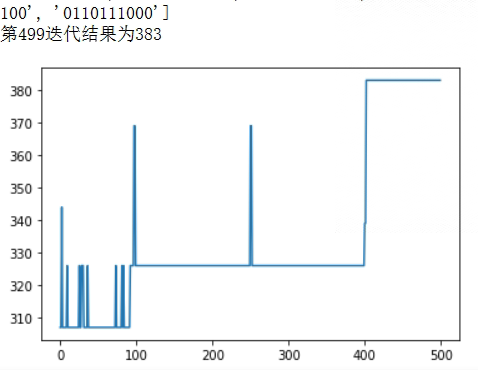
\includegraphics[width=5.0cm]{images/title/sol-1.png}
        }
        \subfloat[第2次运行结果]
        {
          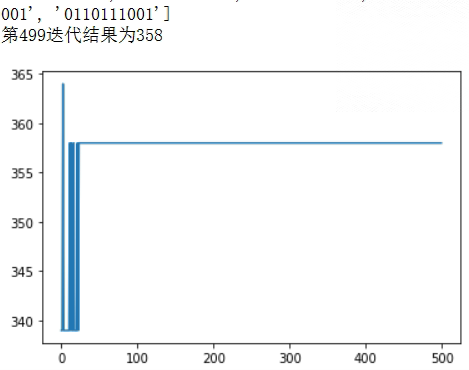
\includegraphics[width=5.0cm]{images/title/sol-2.png}
        }
        \subfloat[第3次运行结果]
        {
          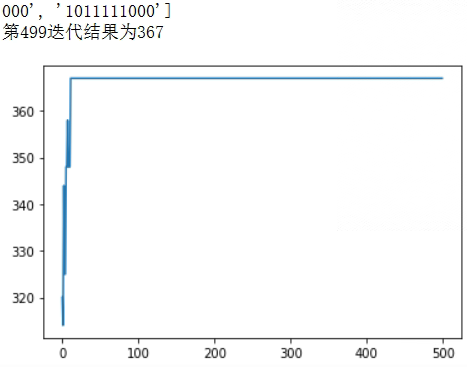
\includegraphics[width=5.0cm]{images/title/sol-3.png}
        }
        
        \subfloat[第4次运行结果]{
          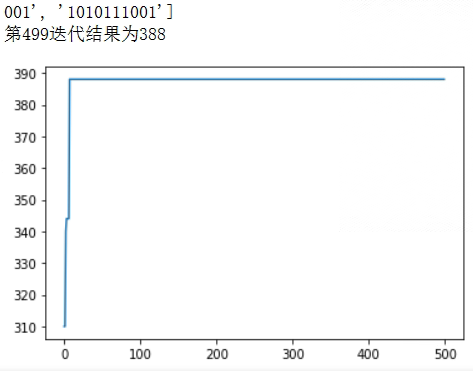
\includegraphics[width=5.0cm]{images/title/sol-4.png}
        }
        \subfloat[第5次运行结果]
        {
          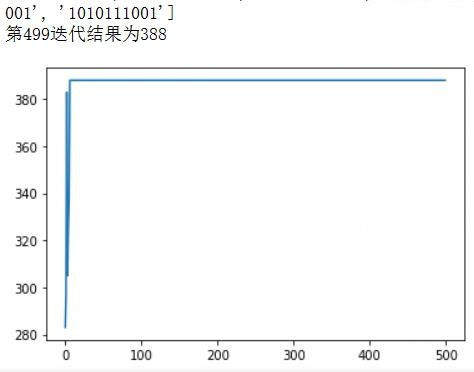
\includegraphics[width=5.0cm]{images/title/sol-5.png}
        }
        \subfloat[第6次运行结果]
        {
          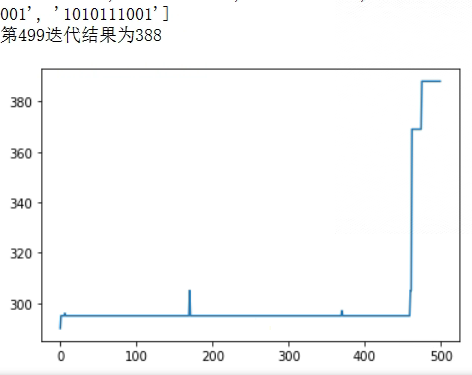
\includegraphics[width=5.0cm]{images/title/sol-6.png}
        }
        \caption{各次的运行结果}
        \label{fig:taizhous}
    \end{figure}
    主函数中的实例的最优解可以用分支限界算法计算出解向量为$X=(1,0,1,0,1,1,1,0,0,1)$, 最优值为388. 上述遗传算法在后3次的运行结果是同正确解相吻合的, 并且上述遗传算法相较于分支限界算法是很快的, 60ms就可以得出结果, 只不过需要多次运行并观察以得出最优解.
\end{homeworkProblem}

\pagebreak

\begin{homeworkProblem}
    上机实现TSP的模拟退火算法, 随机生成一定规模的数据或用通用数据集比较其它人的结果, 分析算法的性能, 摸索实现中技术问题的解决.

    \solution 算法对应的Matlab代码如下所示:
\begin{tcblisting}{listing engine=minted,boxrule=0.1mm,
colback=blue!5!white,colframe=blue!75!black,
listing only,left=5mm,enhanced,sharp corners=all,
overlay={\begin{tcbclipinterior}\fill[red!20!blue!20!white] (frame.south west)
rectangle ([xshift=5mm]frame.north west);\end{tcbclipinterior}},
minted language=matlab,
minted style=tango,
minted options={fontsize=\small,breaklines,autogobble,linenos,numbersep=3mm}}
function D = Distance(citys)
%% 计算两两城市之间的距离
% 输入 citys  各城市的位置坐标
% 输出 D  两两城市之间的距离
n = size(citys,1);
D = zeros(n,n);
for i = 1:n
   for j = i+1:n
       D(i,j) = sqrt(sum((citys(i,:) - citys(j,:)).^2));
       D(j,i) = D(i,j);
   end
end
\end{tcblisting}
\begin{tcblisting}{listing engine=minted,boxrule=0.1mm,
    colback=blue!5!white,colframe=blue!75!black,
    listing only,left=5mm,enhanced,sharp corners=all,
    overlay={\begin{tcbclipinterior}\fill[red!20!blue!20!white] (frame.south west)
    rectangle ([xshift=5mm]frame.north west);\end{tcbclipinterior}},
    minted language=matlab,
    minted style=tango,
    minted options={fontsize=\small,breaklines,autogobble,linenos,numbersep=3mm}}
    function S2 = NewAnswer(S1)
    %% 输入
    % S1:当前解
    %% 输出
    % S2:新解
    N = length(S1);
    S2 = S1;                
    a = round(rand(1,2)*(N-1)+1); %产生两个随机位置 用来交换
    W = S2(a(1));
    S2(a(1)) = S2(a(2));
    S2(a(2)) = W;         %得到一个新路线
\end{tcblisting}
\begin{tcblisting}{listing engine=minted,boxrule=0.1mm,
    colback=blue!5!white,colframe=blue!75!black,
    listing only,left=5mm,enhanced,sharp corners=all,
    overlay={\begin{tcbclipinterior}\fill[red!20!blue!20!white] (frame.south west)
    rectangle ([xshift=5mm]frame.north west);\end{tcbclipinterior}},
    minted language=matlab,
    minted style=tango,
    minted options={fontsize=\small,breaklines,autogobble,linenos,numbersep=3mm}}
    function DrawPath(Route,citys)
    %% 画路径函数
    %输入
    % Route  待画路径   
    % citys  各城市坐标位置
    
    figure
    plot([citys(Route,1);citys(Route(1),1)],...
         [citys(Route,2);citys(Route(1),2)],'o-');
    grid on
    
    for i = 1:size(citys,1)
        text(citys(i,1),citys(i,2),['   ' num2str(i)]);
    end
    
    text(citys(Route(1),1),citys(Route(1),2),'       起点');
    text(citys(Route(end),1),citys(Route(end),2),'       终点');    
\end{tcblisting}
\begin{tcblisting}{listing engine=minted,boxrule=0.1mm,
    colback=blue!5!white,colframe=blue!75!black,
    listing only,left=5mm,enhanced,sharp corners=all,
    overlay={\begin{tcbclipinterior}\fill[red!20!blue!20!white] (frame.south west)
    rectangle ([xshift=5mm]frame.north west);\end{tcbclipinterior}},
    minted language=matlab,
    minted style=tango,
    minted options={fontsize=\small,breaklines,autogobble,linenos,numbersep=3mm}}
function [S,R] = Metropolis(S1,S2,D,T)
%% 输入
% S1:  当前解
% S2:   新解
% D:    距离矩阵(两两城市的之间的距离)
% T:    当前温度
%% 输出
% S:   下一个当前解
% R:   下一个当前解的路线距离
R1 = PathLength(D,S1);  %计算路线长度
N = length(S1);         %得到城市的个数
R2 = PathLength(D,S2);  %计算路线长度
dC = R2 - R1;   %计算能力之差
if dC < 0       %如果能力降低 接受新路线
    S = S2;
    R = R2;
elseif exp(-dC/T) >= rand   %以exp(-dC/T)概率接受新路线
    S = S2;
    R = R2;
else        %不接受新路线
    S = S1;
    R = R1;
end
\end{tcblisting}
\begin{tcblisting}{listing engine=minted,boxrule=0.1mm,
    colback=blue!5!white,colframe=blue!75!black,
    listing only,left=5mm,enhanced,sharp corners=all,
    overlay={\begin{tcbclipinterior}\fill[red!20!blue!20!white] (frame.south west)
    rectangle ([xshift=5mm]frame.north west);\end{tcbclipinterior}},
    minted language=matlab,
    minted style=tango,
    minted options={fontsize=\small,breaklines,autogobble,linenos,numbersep=3mm}}
    function p = OutputPath(R)
    %% 输出路径函数
    % 输入:R 路径
    R = [R,R(1)];
    N = length(R);
    p = num2str(R(1));
    for i = 2:N
        p = [p,'$\to $',num2str(R(i))];
    end
    disp(p)    
\end{tcblisting}
\begin{tcblisting}{listing engine=minted,boxrule=0.1mm,
    colback=blue!5!white,colframe=blue!75!black,
    listing only,left=5mm,enhanced,sharp corners=all,
    overlay={\begin{tcbclipinterior}\fill[red!20!blue!20!white] (frame.south west)
    rectangle ([xshift=5mm]frame.north west);\end{tcbclipinterior}},
    minted language=matlab,
    minted style=tango,
    minted options={fontsize=\small,breaklines,autogobble,linenos,numbersep=3mm}}
    function Length = PathLength(D,Route)
    %% 计算各个体的路径长度
    % 输入:
    % D     两两城市之间的距离
    % Route 个体的轨迹
    
    Length = 0;
    n = size(Route,2);
    for i = 1:(n - 1)
        Length = Length + D(Route(i),Route(i + 1));
    end
    Length = Length + D(Route(n),Route(1));    
\end{tcblisting}
    主函数编码如下:
    \begin{tcblisting}{listing engine=minted,boxrule=0.1mm,
        colback=blue!5!white,colframe=blue!75!black,
        listing only,left=5mm,enhanced,sharp corners=all,
        overlay={\begin{tcbclipinterior}\fill[red!20!blue!20!white] (frame.south west)
        rectangle ([xshift=5mm]frame.north west);\end{tcbclipinterior}},
        minted language=matlab,
        minted style=tango,
        minted options={fontsize=\small,breaklines,autogobble,linenos,numbersep=3mm}}
%% I. 清空环境变量
clear all
clc

%% II. 导入城市位置数据
X = [16.4700   96.1000
     16.4700   94.4400
     20.0900   92.5400
     22.3900   93.3700
     25.2300   97.2400
     22.0000   96.0500
     20.4700   97.0200
     17.2000   96.2900
     16.3000   97.3800
     14.0500   98.1200
     16.5300   97.3800
     21.5200   95.5900
     19.4100   97.1300
     20.0900   92.5500];

%% III. 计算距离矩阵
D = Distance(X);  %计算距离矩阵
N = size(D,1);    %城市的个数

%% IV. 初始化参数
T0 = 1e10;   % 初始温度
Tend = 1e-30;  % 终止温度
L = 2;    % 各温度下的迭代次数
q = 0.9;    %降温速率
syms x;
Time = ceil(double(solve(T0*(0.9)^x == Tend)));    % 计算迭代的次数
% Time = 132;
count = 0;        %迭代计数
Obj = zeros(Time,1);         %目标值矩阵初始化
track = zeros(Time,N);       %每代的最优路线矩阵初始化

%% V. 随机产生一个初始路线
S1 = randperm(N);
DrawPath(S1,X)
disp('初始种群中的一个随机值:')
OutputPath(S1);
Rlength = PathLength(D,S1);
disp(['总距离:',num2str(Rlength)]);

%% VI. 迭代优化
while T0 > Tend
    count = count + 1;     %更新迭代次数
    temp = zeros(L,N+1);
    %%
    for k = 1:L
        % 1. 产生新解
        S2 = NewAnswer(S1);
    \end{tcblisting}
\begin{tcblisting}{listing engine=minted,boxrule=0.1mm,
colback=blue!5!white,colframe=blue!75!black,
listing only,left=5mm,enhanced,sharp corners=all,
overlay={\begin{tcbclipinterior}\fill[red!20!blue!20!white] (frame.south west)
rectangle ([xshift=5mm]frame.north west);\end{tcbclipinterior}},
minted language=matlab,
minted style=tango,
minted options={fontsize=\small,breaklines,autogobble,linenos,numbersep=3mm}}
         % 2. Metropolis法则判断是否接受新解
         [S1 R] = Metropolis(S1, S2, D, T0);   % Metropolis抽样算法
         temp(k, :) = [S1 R];            % 记录下一路线及其长度
     end
     %% 3. 记录每次迭代过程的最优路线
     [d0, index] = min(temp(:, end));    % 找出当前温度下最优路线
     if count == 1 || d0 <= Obj(count-1)
         Obj(count) = d0;                    % 如果当前温度下最优路程小于上一路程则记录当前路程
     else
         Obj(count) = Obj(count-1);    % 如果当前温度下最优路程大于上一路程则记录上一路程
     end
     track(count, :) = temp(index, 1:end-1);  % 记录当前温度的最优路线
     %降温
     T0 = q * T0;
 end
 
 %% VII. 优化过程迭代图
 figure
 plot(1:count,Obj)
 xlabel('迭代次数')
 ylabel('距离')
 title('优化过程')
 
 %% VIII. 绘制最优路径图
 DrawPath(track(end,:),X)
 
 %% IX. 输出最优解的路线和总距离
 disp('最优解:')
 S = track(end,:);
 p = OutputPath(S);
 disp(['总距离:',num2str(PathLength(D,S))]);
\end{tcblisting}
    优化前的一个随机路线轨迹图如图\ref{fig:随机路线图}所示:
    \begin{figure}[H]  % 这里记得用[H]
        \centering
        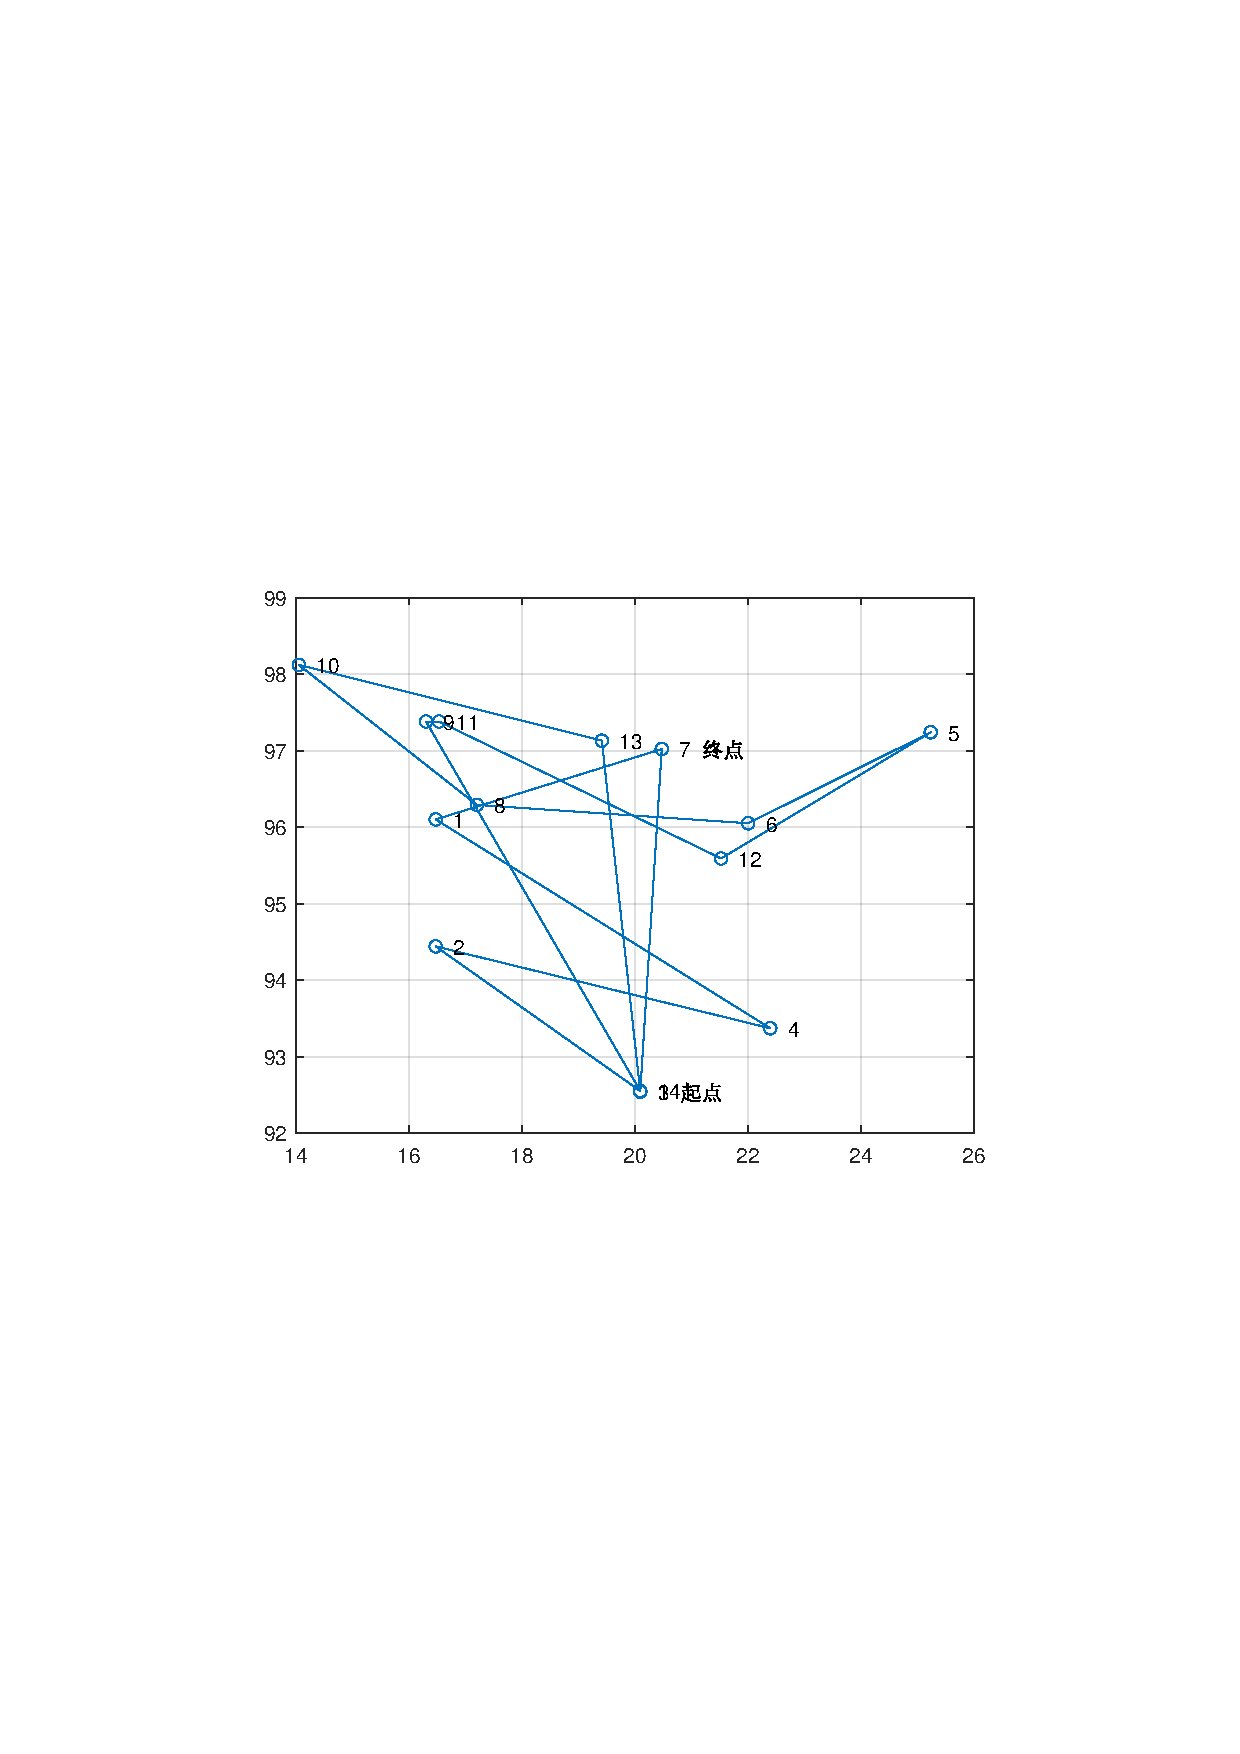
\includegraphics[width=0.55\linewidth]{images/title/随机路线图.pdf}
        \caption{随机路线图}
        \label{fig:随机路线图}
    \end{figure}
    初始种群中的一个随机值: 5$\to $12$\to $6$\to $11$\to $7$\to $13$\to $10$\to $4$\to $8$\to $9$\to $3$\to $2$\to $14$\to $1$\to $5, 
    
    总距离为66.0171. 优化后的路线如图\ref{fig:最优解路线图}所示:
    \begin{figure}[H]  % 这里记得用[H]
        \centering
        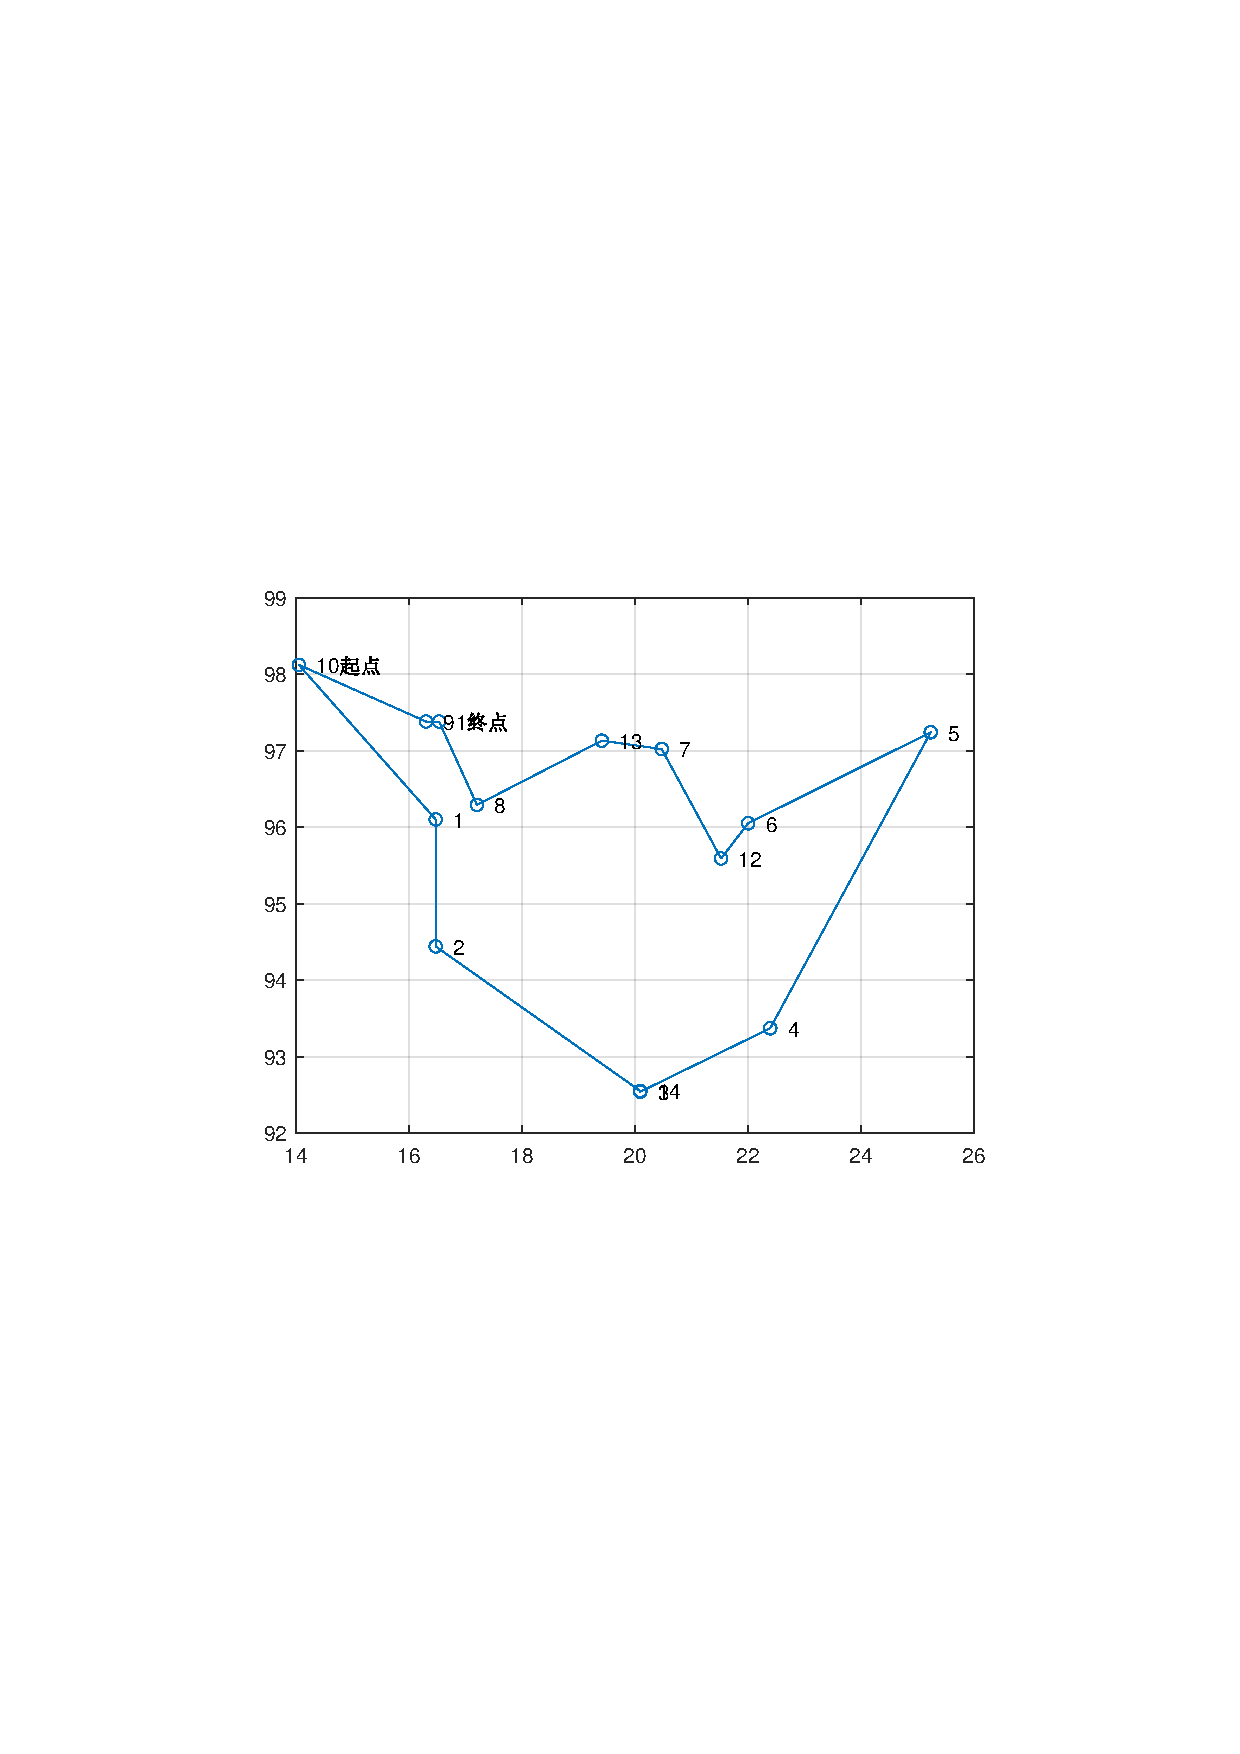
\includegraphics[width=0.55\linewidth]{images/title/最优解路线图.pdf}
        \caption{最优解路线图}
        \label{fig:最优解路线图}
    \end{figure}
    最优解: 6$\to $12$\to $7$\to $13$\to $8$\to $11$\to $9$\to $10$\to $1$\to $2$\to $14$\to $3$\to $4$\to $5$\to $6, 总距离为29.3405. 优化迭代过程如下图\ref{fig:模拟退火算法优化过程图}所示:
    \begin{figure}[H]  % 这里记得用[H]
        \centering
        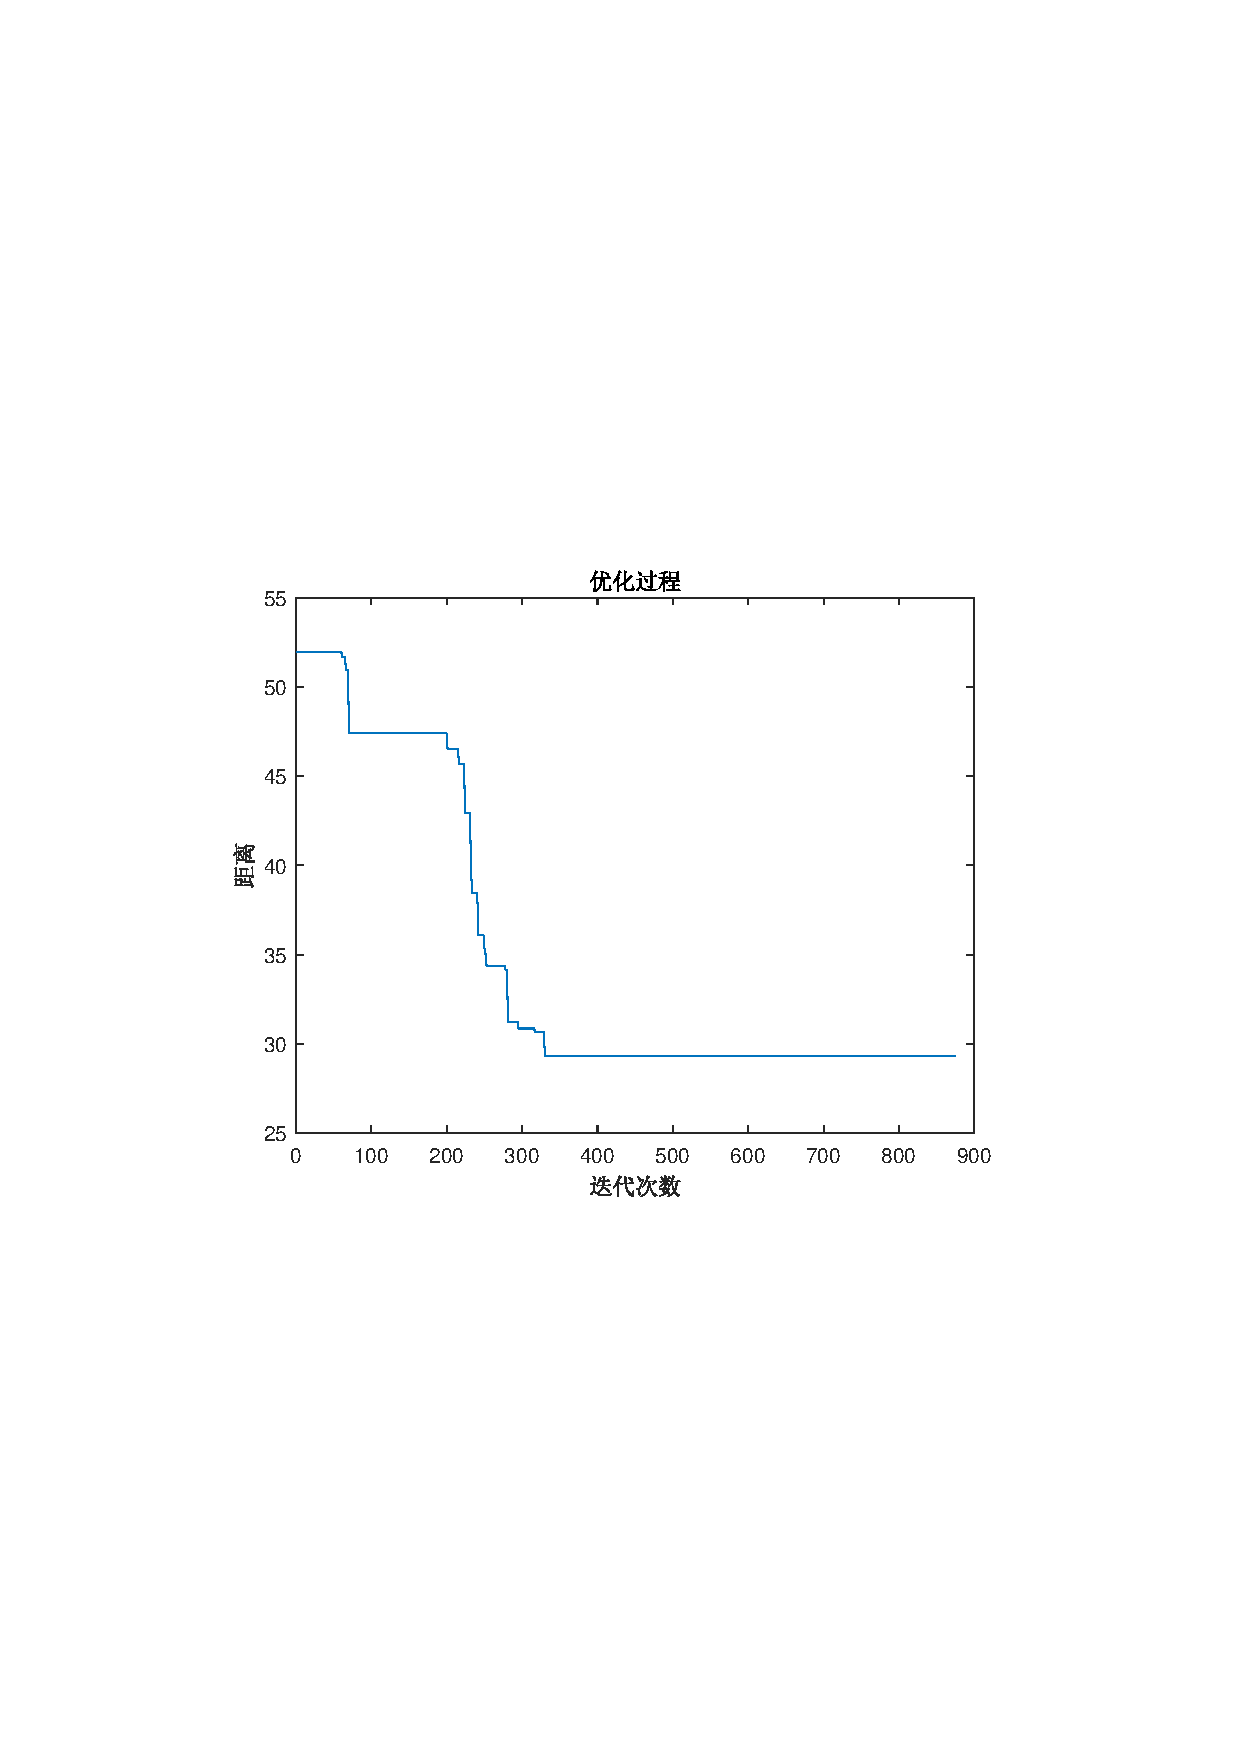
\includegraphics[width=0.55\linewidth]{images/title/模拟退火算法优化过程图.pdf}
        \caption{模拟退火算法优化过程图}
        \label{fig:模拟退火算法优化过程图}
    \end{figure}
    由上图可以看出: 优化前后路径长度得到很大改进, 由优化前的66.0171变为29.3405, 变为原来的44.4\%, 400多代以后路径长度已经保持不变了, 可以认为已经是最优解了.
\end{homeworkProblem}


\begin{figure}[H]  % 这里记得用[H]
    \centering
    
\includegraphics[width=0.5\linewidth]{images/title/ucas_logo 1.pdf}
    %\caption{ucas-logo}
    \label{fig:ucas-logo}
\end{figure}

% 引用文献
\bibliographystyle{unsrt}  % unsrt:根据引用顺序编号
\bibliography{refs}


\end{document}
